\part{Viengoos}

\chapter{Designation}

\begin{quotation}
  ``The name of the song is called `HADDOCKS' EYES.'\,''

  ``Oh, that's the name of the song, is it?'' Alice said, trying to feel
  interested.

  ``No, you don't understand,'' the Knight said, looking a little vexed.
  ``That's what the name is CALLED.  The name really IS `THE AGED AGED
  MAN.'\,''

  ``Then I ought to have said `That's what the SONG is called'?''
  Alice corrected herself.

  ``No, you oughtn't: that's quite another thing!  The SONG is called
  `WAYS AND MEANS': but that's only what it's CALLED, you know!''

  ``Well, what IS the song, then?'' said Alice, who was by this
  time completely bewildered.

  ``I was coming to that,'' the Knight said.  ``The song really IS
  `A-SITTING ON A GATE':  and the tune's my own invention.''

  \begin{flushright}
    \emph{Through the Looking Glass}\\
    Lewis Carroll
  \end{flushright}
\end{quotation}


Viengoos is an object-capability system.  Objects are designated
exclusively by way of capabilities, which are kernel-protected,
unforgeable references.  Capabilities are in turn designated by
indexing an address space.  Each thread object has a capability slot
that identifies the root of its address space.  When a thread invokes
an object, it specifies an index.  Viengoos finds the capability
corresponding to this index in its address space and then dereferences
the capability to obtain the object.

This chapter first describes how capabilities work, their format, and
the kernel supported methods for manipulating capabilities.  We then
discuss addressing.  Namely, how addresses are encoded, address space
construction, and address resolution.

\section{Capabilities}

A capability both \emph{designates} an object and \emph{authorizes}
access to it.  (The importance of this is best illustrated by the
Confused Deputy problem \cite{hardy88confused-deputy}.)  Capabilities
are unforgeable in that they are kernel protected---their bit
representation is never exposed---and thus can only be transferred via
authorized channels.

To sense or modify an object, a thread may \emph{invoke} it.
Invocation causes a message to be sent to the object.  The exact
semantics of an invocation depend on the invoked object's
implementation.

A capability may be delegated by transferring it in an object
invocation.  When a capability is transferred in such a way, the
capability is copied to the receipient's message buffer.  Because the
receive buffer is allocated beforehand, copying does not require that
the kernel allocate memory.

In Viengoos, the only way to revoke access to an object is to destroy
the object.\footnote{Revocation can be implemented by way of Redell's
  Caretaker but so far, this mechanism has not been required.}  By
destroying the object, all capabilities designating it become invalid
and act as if they designated the VOID object.

Viengoos allows user-object implementations.  A user object is
implemented by a process.  The process allocates an end point and
delegates it to clients.  To use the object, a client invokes the end
point.  The server process is then notified that there is a message
and may act on it as it sees fit.

As user objects are accessed in the same way as kernel objects, it is
possible to interpose on specific objects or to fully or partially
emulate the kernel from a user-space process.

\subsection{Format}

A capability is 128-bits wide and consists of the following fields:

\begin{itemize}
\item an object identifier (OID),
\item a version,
\item a weak predicate (W),
\item address translation directives,
  \begin{itemize}
  \item a guard, and
  \item a sub-page descriptor
  \end{itemize}
\item an object memory policy,
  \begin{itemize}
  \item a discardability predicate (D), and
  \item a priority
  \end{itemize}
\end{itemize}

\subsubsection{Object Identification}

The OID field is used to locate an object.  The OID corresponds to a
block of storage on backing store.  Backing store is managed by
so-called backing store managers.  When an object is referenced and
the object is not in memory, Viengoos submits a request to page the
object in to the appropriate backing store manager.  Similarly, when
Viengoos decides that the object should be flushed to persistent
store, it sends a request to the backing store manager.

When an object is destroyed, all references to it must be invalidated.
Invalidating references is difficult as it requires finding all of the
references.  Maintaining a linked list of capabilities referencing an
object requires two additional pointers per capability.  But this only
suffices for in-memory objects: if a cappage is paged-out and the
object is destroyed, these must be invalidated as well.  To work
around this problem, each object also has a version number.  When a
capability to an object is created, the object's version number is
copied into the capability.  Then, when dereferencing a capability,
the capability is only considered valid if the the version numbers
match.  If they do not match, then the reference is known to not be
valid and the VOID object is returned instead of the object instance.

The use of the version field raises another problem: it is limited in
size.  To avoid overflowing it and having to do a disk scavenge before
being able to reuse the storage, it is imperative to control its
growth.  The solution EROS has used is to only bump the field if a
capability designating the object goes to disk, a relatively rare
occurrence, they observe, and to rate-limit that to once every few
minutes \cite{citation-needed}.

\subsubsection{Weak Capabilities}

The data, cappage, endpoint, and activity objects implement two
interfaces (facets): a so-called strong facet and a weak facet.  The
weak facet allows access to a subset of the functionality that the
strong facet allows.

A capability designating the weak facet of a data-page provides
read-only access to the object.  The same applies for a cappage,
however, the access is transitively removed: strong capabilities
fetched via a weak capability are downgraded by the kernel to weak
reference the object's weak facet.  A capability designating the weak
facet of an end-point only allows enqueuing messages.  And, a
capability designating the weak facet of an activity does not allowing
changing the activity's policy.

\subsubsection{Address Translation}

In Viengoos, address spaces are composed through the arrangement of
cappages; cappages act as page-tables.  A thread object contains a
capability slot, which is filled with the root capability.  Some
object methods all take a capability designating the root.

Viengoos uses a guarded page table scheme
\cite{liedtke94page-table-structures-for-fine-grain-vm}.  To support
this, capabilities contain two fields: a guard and a subpage
descriptor.  The guard consists of a value and a length.  A subpage
descriptor allows the use of only part of a capability page in address
translation.  It consists of a subpage count and an offset.  The count
indicates the number of subpages in the cappage.  This value must be
between 1 and 256 inclusive and be a power of 2.  For example, a count
of 2 means to divide the cappage into two subpages, each consisting of
$256 / 2 = 128$ capabilities.  The offset is then used to select the
subpage to index.  Address translation is discussed in section
\ref{address-translation}.

\subsubsection{Object Memory Policy}

To allow principals to control memory is managed, each capability
contains two fields that describe the discardability and the priority
of the designated object.  Resource management is described in
chapter~\ref{chapter:resource-management}.

\section{Addressing}

Capabilities designated using thread-local addresses.  Each thread
object contains a capability slot that identifies the root of its
address space.  To designate a capability, a thread specifies the
index of the capability in this address space.

\subsection{Address Encoding}

On Viengoos, all addresses are 64-bits wide.  This is true even on
32-bit platforms.  On these platforms, hardware addresses are
automatically extended.

A Viengoos address consists of a {\bf prefix} and a {\bf depth}.  The
depth specifies the length of the prefix.  This type of addressing
allows addressing not only leaf objects but also internal nodes.  (The
intuition behind an addresses depth is how far into the tree to
search.)  The address prefix is encoded in the most significant bits
of the address.  This is followed by a bit with the value of 1, and
then $63 - depth$ (\var{idepth}), which is encoded in unary.

\begin{center}
  \begin{bytefield}{32}
    \tiny{63}\hspace{\stretch{1}}\tiny{0}\\
    \bitsl{20}{depth}{prefix} & \bit{1} & \bitsl{11}{63 - depth}{idepth}
  \end{bytefield}
\end{center}

Observe that the value of idepth is the position of the least
significant bit that is on.

The address with all zeros is the NULL address.  The NULL address is
sometimes used to denote some default action.  When returned, it
typically means failure.

By convention, addresses are written \emph{prefix/depth}.

Viengoos automatically translates machine addresses to the above form.
The prefix is set to the machine address zero-extended to 63 bits and
the depth is set to 63.  For machines with 64-bits addresses,
addresses with the most significant bit set are illegal.

The root capability slot is identified by the address 0/0.  Its
encoding is:

\begin{center}
  \begin{bytefield}{32}
    \tiny{63}\hspace{\stretch{1}}\tiny{0}\\
    \bit{1} & \bitsl{31}{63}{0}
  \end{bytefield}
\end{center}

The address 0x804b2c0 is encoded:

\begin{center}
  \begin{bytefield}{32}
    \tiny{63}\hspace{\stretch{1}}\tiny{0}\\
    \bitsl{31}{63}{0x804b2c0} & \bit{1}
  \end{bytefield}
\end{center}

The address of the data object that contains the above byte would be
the address rounded down to the nearest page size and with a depth of
63 - the logarithm base 2 of the page size.  If the underlying
hardware has base pages with a size of 4kb, then the address would be
0x804b000/51.


\subsection{Address Translation}
\label{address-translation}

\begin{algorithm}
\begin{algorithmic}[1]
\Function{Thread $\rightarrow$ CapabilitySlotLookup}{$\mathit{address}$}
  \State $C \gets \mathit{thread.root}$
  \Comment{The root of the address space.}
  \State $P \gets \mathit{prefix}(\mathit{address})$
  \Comment{The bits to translate.}
  \State $R \gets \mathit{depth}(\mathit{address})$
  \Comment{The number of bits remaining.}
  \Statex

  \Loop
  \If {$R = 0$} \label{alg:before-guard-check-start}
    \State \Return $\&C$
    \Comment{C is the designated capability.}
  \EndIf \label{alg:before-guard-check-end}
  \Statex

  \BigComment{Check the guard.}
  \If{$R < \mathit{guard\_length}(C)$} \label{alg:guard-compare-start}
    \State \Return failure
    \Comment{Not enough bits to translate guard.}
  \EndIf
  \If {$\mathit{guard}(C) \not= P_{R..R-\mathit{guard\_length}(C) + 1}$}
    \State \Return failure
    \Comment{The guard does not match.}
  \EndIf
  \State $R \gets R - \mathit{guard\_length}(C)$ \label{alg:guard-compare-end}

  \Statex
  \If {$R = 0$} \label{alg:after-guard-check-start}
    \State \Return $\&C$
    \Comment{C is the designated capability.}
  \EndIf \label{alg:after-guard-check-end}

  \Statex
  \State $\triangleright$ Look up the object designated by the PTE.
  \State $O \gets \mathit{cap\_to\_object}(C)$ \label{alg:object-lookup}
  \If{$\neg O \mathit{or} \mathit{typeof} (O) \not= cappage$}
    \State \Return failure \Comment{Type mismatch.}
  \EndIf

  \Statex
  \State $\triangleright$ Index the capability page getting the next
  page table entry.
  \State $S \gets 256/\mathit{subpages}(C)$ \Comment{The subpage size.}
  \label{alg:subpage-index-start}
  \If {$R < log_2(S)$}
    \State \Return failure
    \Comment{Not enough bits to index the cappage.}
  \EndIf

  \State $C \gets
    O.\mathit{caps}\left[S/\mathit{subpages}(C)
    + P_{R..R-\log_2(S)+1}\right]$

  \State $R \gets R - \log_2(S)$ \label{alg:subpage-index-end}
\EndLoop
\EndFunction
\end{algorithmic}
\caption{Capability slot lookup.}
\label{alg:capability-lookup}
\end{algorithm}

\begin{figure}
  \begin{center}
    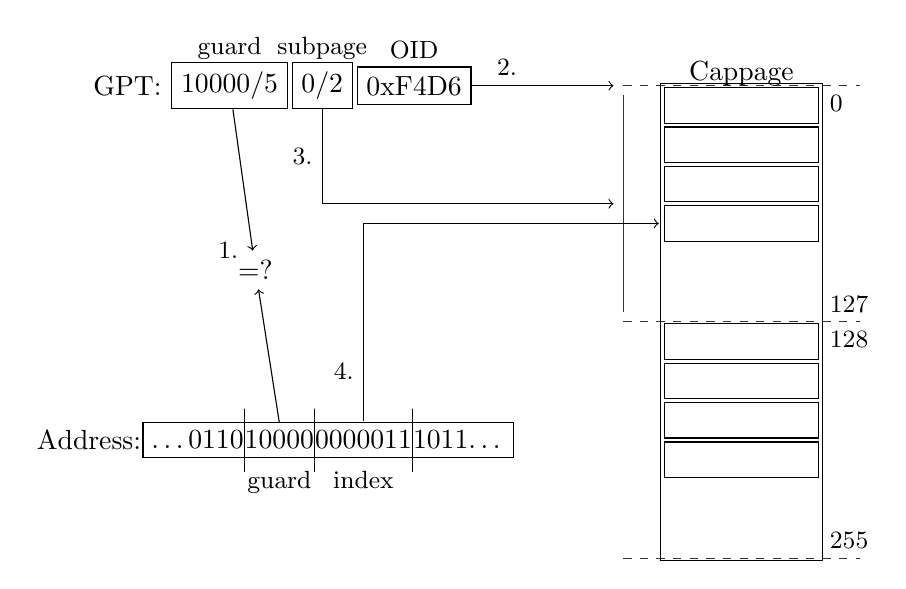
\begin{tikzpicture}
      % Draw a capability page on the right.
      \begin{scope}[shift={(6.5,0)}]
        \draw[dashed,black!80] (-0.5,0) -- +(3,0)
          (-0.5,3) node (subpage1) {} -- +(3,0)
          (-0.5,6) node (subpage0) {} -- +(3,0);

        \draw (-0.025,-0.025) rectangle +(2.05,6.05);

        % Each slot is 2x0.5.  We leave 0.025 white space around the
        % outline shape thus imply 0.05 white space between objects.
        \foreach \s in {2,3,...,5,8,9,...,11}
          \draw (0, \s/2)
            +(1,0.25) node (slot\s) {}
            ++(0.025,0.025) rectangle +(1.95,0.45);

        \path (2,6) node[anchor=north west] {\small{0}}
              ++(0,-3) node[anchor=south west] {\small{127}}
              ++(0,0) node[anchor=north west] {\small{128}}
              ++(0,-3) node[anchor=south west] {\small{255}};

        \node[anchor=south] at (slot11.north) {Cappage};
      \end{scope}

      % Draw the address.

      % The address.
      \path[inner sep=0] node (apre) [anchor=west] at (0,1.5) {\ldots0110}
        (apre.east) node (ag) [anchor=west] {10000}
        (ag.east) node (ai) [anchor=west] {0000011}
        (ai.east) node (apost) [anchor=west] {1011\ldots};

      % The bounding box.
      \path (apre.north west) +(-0.1,0.1) node (a_tl) {};
      \path (apost.south east) +(0.1,-0.1) node (a_br) {};
      \draw (a_tl) rectangle (a_br);

      % Vertical separators.
      \foreach \h in {0.8}
      {
        \draw (apre.east) -- +(0, \h / 2) -- +(0, -\h / 2);
        \draw (ag.east) -- +(0, \h / 2) -- +(0, -\h / 2);
        \draw (ai.east) -- +(0, \h / 2) -- +(0, -\h / 2);
      }

      % The labels.
      \path (ag.south) +(0,-0.5) node[anchor=base] {\small guard}
        (ai.south) +(0,-0.5) node[anchor=base] {\small index};


      % Draw the capability.

      \draw (1,6) node[draw] (guard) {10000/5}
        (guard.east) +(0.05,0) node [draw,anchor=west] (subpage) {0/2}
        (subpage.east) +(0.05,0) node [draw,anchor=west] (oid) {0xF4D6};

      \path (guard.north) +(0,0.1) node[anchor=base] {\small guard}
        (subpage.north) +(0,0.1) node[anchor=base] {\small subpage}
        (oid.north) +(0,0.1) node[anchor=base] {\small OID};


      % Connect the dots.
      \draw[->] (oid.east) -- node [near start, above] {\small 2.} (subpage0);

      \draw[black!80] (subpage0) -- node (subpage0mid) {} (subpage1);
      \draw[->] (subpage.south) |- node [near start, left] {\small 3.} (subpage0mid);

      \path (guard) -- node (compare) {=?} (ag);
      \draw[->] (guard) -- (compare);
      \draw[->] (ag.north) +(0,0.1) -- (compare);
      \node at (compare.north west) {\small 1.};

      \draw[->] (ai.north) +(0,0) node (ain) {}
        (slot8.west) ++(-0.8,0) node (slot8w) {}
        (ain) |- node [very near start, left] {\small 4.} (slot8w);

      \node[anchor=east] at (guard.west) {GPT:};
      \node[anchor=east] at (apre.west) {Address:};

    \end{tikzpicture}
  \end{center}
  \caption[Address translation using guard page tables]{Translating
    part of an address using a GPT entry.  The capability containing
    the GPT entry is at the top left in the figure, to the right is
    the referenced capability page, and bottom left is the address.
    First, the guard is compared to the address.  If they match, the
    object is found.  The subpage descriptor selects a part of the
    capability page, which is then indexed using the next portion of
    the address.}
  \label{fig:address-translation}
\end{figure}

\index{address translation!algorithm|(}

Address translation proceeds according to the following algorithm.
Given an address, translation starts with the capability in the
thread's address space capability slot.  First, the most significant
bits of the address are compared with the guard in the capability
(lines \ref{alg:guard-compare-start}--\ref{alg:guard-compare-end}).
If these match, those address bits are consumed.  If there are no
address bits left, then the designated capability slot has been
located and is returned.  Otherwise, the object designated by the
capability is found (line \ref{alg:object-lookup}), divided according
to the subpage descriptor in the capability and indexed using the most
significant remaining bits of the address (lines
\ref{alg:subpage-index-start}--\ref{alg:subpage-index-end}).  Again,
the number of bits used to index the subpage are consumed.  If all the
bits are consumed, the capability slot has been located and is
returned.  Otherwise, the process is repeated with the new capability
and the remaining address bits.  An iteration of this process is
illustrated in figure~\ref{fig:address-translation}.

Note that a capability slot can be identified by two different names:
either with or without the guard specified in the slot.  This is a
matter of convenience: it is useful to be able to modify the
capability that designates the object at a particular address by
designating the object.  If this functionality were not provided,
doing this would require finding the guard, which is possible but
cumbersome.  Moreover, the extension is quite simple.

When looking up objects, the same principle applies, however, the
check if the address has been fully translated at
lines~\ref{alg:before-guard-check-start}--\ref{alg:before-guard-check-end}
is removed.  That is, it is not sufficient to specify the capability
slot that designates the object, the guard must also match.

\index{address translation!algorithm|)}

\section{Data Structures}

\subsection{\type{addr}}

The format of an address is:

\begin{center}
  \begin{bytefield}{32}
    \tiny{63}\hspace{\stretch{1}}\tiny{0}\\
    \bit{1} & \bitsl{31}{63}{0}
  \end{bytefield}
\end{center}

\var{idepth} is stored in unary.  The depth is 63 - \var{idepth}.

\subsection{\type{addr_trans}}

The \type{addr_trans} structure has the following layout:

\begin{struct}{32}
  \bitsl{14}{22-lsp}{guard}
  & \bitsl{8}{(lsp)}{subpage}
  & \bits{4}{$log_2$ sps}
  & \bits{6}{g\_depth}
\end{struct}

\var{$log_2$ sps} is logarithm base 2 of the number of subpages.
\var{subpage} is the subpage to select.  It has a width of \var{lsp}.
\var{g\_depth} is the number of length of the guard.  \var{guard} is
the value of the guard and is zero-extended to \var{g\_depth}.  Its
width is also not fixed.

\subsection{\type{object_policy}}

The \type{object_policy} structure has the following layout:

\begin{struct}{8}
  \bit{D} & \bits{7}{priority}
\end{struct}

\var{D} is the discardability predicate.

\subsection{\type{cap_properties}}

The \type{cap_properties} structure has the following layout:

\begin{struct}{32}
  \bits{24}{\dontcare} & \bits{8}{object\_policy} \\
  \bits{32}{addr\_trans}
\end{struct}

\subsection{\type{cap}}

The following is the internal representation of a capability.  Only
the discardability predicate, the priority and the address translator
are exposed to the user.

\begin{struct}{32}
  \bits{23}{version} & \bit{W} & \bit{D} & \bits{7}{priority} \\
  \bits{32}{address translator} \\
  \wordbox{2}{OID}
\end{struct}

\var{D} is the discardability predicate.  \var{W} is the weak
predicate.

\chapter{Resource Management}
\label{chapter:resource-management}

\section{Object Policy}

When an object is accessed, if the object is
claimed,\footnote{Claiming is discussed in \ref{object-claiming}.} the
policy in the designating object is applied to the object.

The discardability property is a hint that Viengoos may, instead of
flushing changes to disk, simply discard a frame's content.  If a
capability has the weak predicate set, this hint is ignored.  If
content discarded, the next access to the object will raise a
discarded event.  If an activity is discarded, all objects allocated
against the activity are destroyed.

The priority property allows an activity to control the order in which
the frames, which it has claimed, are released.  If the content is
dirty and has not been marked as discardable, the content is written
to backing store.  Otherwise, the frame is made eligible for immediate
reuse.

The lower the numric value of the priority field, the lower the
frame's priority.  Frames are released in priority order.  If multiple
frames have the same priority, they are released in a random order
unless the priority is 0, in which case, the frames are released in
approximately LRU order.

%%%%%%%%%%%%%%%%%%%%%%%%%%%%%%%%%%%%%%%%%%%%%%%%%%%%%%%%%%%%%%%%

\chapter{Threads}

A thread encapsulates an execution context.  This consists of a
register file, a name space, and a resource principal.

Viengoos does not implement a first-class task abstraction, which
encapsulates multiple threads running in a single address space.  It
is possible to achieve this on Viengoos by specifying the same address
space root for multiple thread objects.

In Viengoos, unlike in traditional kernels, threads are not blocking
entities.  Blocking is instead done by messengers, which hold and
transfer messages (see chapter~\ref{messengers} for a description of
messengers).  By separating messengers from threads, it is possible to
reliably wait for multiple events while the thread continues to
execute and to do so in a manner that does not require the kernel or a
server to block on the thread.

\section{Thread State}

A thread consists of four user-accessible capability slots: the
address space root, the current activity the exception messenger and
the user-thread control block (UTCB).

A thread object also contains space to save its CPU state, which it
contains when the thread is not executing on a CPU.

\subsection{Address Space Root}

The address space root capability slot determines the root of a
thread's address space.  This address space is used in two situations.
First, when a thread performs an IPC, the arguments are identified by
addresses, which are resolved in this address space.  Second, this
naming context determines the hardware address space.  That is, it is
the context in which the memory addresses to all hardware load and
store instructions are resolved.

\subsection{Activity}

A thread's activity slot determines the thread's current activity.
This is used to schedule the thread and to account resources that are
allocated or consumed when resolving a page fault.

If the activity slot does not contain a capability designating an
activity, the thread is not scheduled.

\subsection{Exception Messenger}

When a thread generates an exception, for instance, when it attempts
to access a memory location for which there is no valid translation,
the thread is suspended, and an exception message is generated and
delivered to the thread's exception messenger.  The kernel delivers
execptions in non-blocking mode meaning if the exeception messenger is
not ready to receive a message, the message is dropped.

\subsection{User-Thread Control Block}

\begin{lstlisting}[float,caption=The user-thread control block structure.,frame=single,captionpos=b]
struct utcb {
  union {
    struct {
      uintptr_t activated_mode : 1;
      uintptr_t pending_message : 1;
      uintptr_t interrupt_in_transition : 1;
    };
    uint64_t status;
  };

  uintptr_t saved_ip;
  uintptr_t saved_sp;

  uintptr_t activation_handler_sp;
  uintptr_t activation_handler_ip;
  uintptr_t activation_handler_end;

  uint64_t protected_payload;
  uint64_t messenger_id;

  /* Inline data.  */
  struct {
    uintptr_t inline_word_count : 2;
    uintptr_t inline_cap_count : 1;
  };
  uintptr_t inline_words[2];
  addr_t inline_caps[1];
};
\end{lstlisting}

The user-thread control block (UTCB) is a normal data page.  It
provides a conduit for the user and kernel to communicate and
coordinate action.  This is primarily used for managing activations
and in message delivery.

\begin{description}

\item[activated mode]

The \var{activated mode} bit indicates whether the thread is in
activated mode.  An activation is only delivered if this bit is clear.
Before a thread is activated, this bit is checked.  If it is set, the
activation is either delayed or dropped.  In the former case, the
messenger causing the activatation blocks on the thread.  A blocked
messenger may be unblocked either by a future activation or if
\func{thread\_activation\_collect} is called.  If the messenger is
destroyed or the delivery aborted, the activation will not be
delivered.

\item[pending message]

The kernel sets the \var{pending message} bit when a messenger
attempts to deliver a message to the thread, however, the thread is in
activated mode.

\item[interrupt in transition]

The \var{interrupt in transition} bit is set by the kernel when
activating a thread to indicate whether the thread was activated while
the instruction pointer was in the so-called \emph{activation
  transition range} (see \var{activation handler start} and
\var{activation handler end} below).

\item[saved ip \textmd{and} saved sp]

When delivering an activation, the kernel interrupts the thread, sets
the \var{saved ip} and \var{saved sp} variables to the instruction
pointer and the stack pointer, sets the thread's sp and ip to
\var{activation handler sp} and \var{activation handler ip},
respecitve, and then resumes the thread.

\item[activation handler sp \textmd{and} activation handler ip]

When the kernel activates a thread, it sets its SP and IP to these
values, respectively.

\item[activation handler ip \textmd{and} activation handler end]

These variables determine the so-called \emph{activation transition
  range}.

If the kernel activates a thread and its in the activation transition
range (between \var{activation handler ip} inclusive and
\var{activation handler end} exclusive, the kernel does not save the
current IP and SP in \var{saved ip} and \var{saved sp} but sets the
\var{interrupt in transition} bit.  Using this mechanism, on many
architectures, it is possible to atomically, with respect to
activation delivery, clear \var{activated mode} and restore the
interrupted stack pointer and instruction pointer without entering the
kernel

\item[protected payload]

When delivering a messenger's message, the \var{protected payload}
variable is set to the protected payload of the capability that was
used to invoke the messenger to send the message.

\item[messenger id]

When delivering a messenger's message, the \var{messenger id} is set
to the messenger's \var{message id}.

\item[inline word count, inline cap count, inline words \textmd{and}
  inline caps]

When a messenger delivers a message inline, \var{inline word count} is
set to the number of words (not bytes) that were transferred and
\var{inline cap count} to the number of capabilities transferred.  The
\var{inline words} variable is filled with any data.  If the message
includes capabilities, they are saved sequentially in the slots
specified at invocation time and the address is copied to \var{inline
  capability}.  If an error occurs while transferring a capability,
the corresponding elemeent in \var{inline capabilities} is set to
\const{ADDR\_VOID}.

\end{description}

\section{Activations}

A thread may be activated if a messenger associated with the thread
transfers or receives a message.  Threads are only activated by
messengers and scheduling events.  In the case of scheduling events, a
kernel-provided messenger whose \var{message id} variable is set to
\const{\~0ULL} is used and delivery is done in a non-blocking manner.

Activating a thread proceeds as follows:

\begin{itemize}
\item Atomically, with respect to the thread's execution:
  \begin{itemize}
  \item If the thread is activated (\var{activated mode} is non-zero):
    \begin{itemize}
    \item If delivery is non-blocking, return.
    \item Otherwise:
      \begin{itemize}
      \item Block the messenger on the thread, and
      \item Set \var{pending message} to $1$.
      \end{itemize}
    \end{itemize}
  \end{itemize}

\item Suspend the thread's execution.

\item Set \var{protected payload} to that saved in the messenger.
\item Set \var{messenger id} to the messenger's messenger id.

\item If the activation is the result of a message receipt:
  \begin{itemize}
  \item If the message is inline:
    \begin{itemize}
    \item Copy the messenger's data to \var{inline words} and
      \var{inline caps}
    \item Update \var{inline word count} and \var{inline cap count}.
    \end{itemize}
  \end{itemize}

\item Set \var{activated mode} to $1$.

\item If the thread's IP is between \var{activation handler ip}
  (inclusive) and \var{activation handler end} (exclusive):
  \begin{itemize}
  \item Set \var{interrupt in transition} to $1$.
  \end{itemize}
\item Otherwise:
  \begin{itemize}
  \item Set \var{interrupt in transition} to $0$,
  \item Set \var{saved sp} to the thread's stack pointer, and
  \item Set \var{saved ip} to the thread's instruction pointer.
  \end{itemize}

\item Set the thread's stack pointer to \var{activation handler sp}.
\item Set the thread's instruction pointer to \var{activation handler
  ip}.

\item Resume the thread.

\end{itemize}

\section{Exceptions}

Exceptions are synthesized by the kernel in response to a thread
action.  There is one type of exception, a fault exception.

The following actions result in the generation of a fault exception:

\begin{description}
\item[page fault] A hardware load or store attempts to dereference an
  address for which there is no valid translation.
\item[access fault] A hardware load or store attempts to accesses an
  object in an unauthorized manner.
\item[discarded] A hardware load or store attempts to access an object
  that has been discarded.
\end{description}

When a thread generates an exception, the thread is suspended and a
fault message is delivered to its exception messenger.  If this would
block, the message is discarded.

A fault message takes four parameters: the address of the fault (using
Viengoos address encoding), the value of the stack pointer, the value
of the instruction pointer and a fault information structure, which
includes the type of access and whether the object has been discarded:

\begin{center}
  \begin{bytefield}{32}
    \tiny{63}\hspace{\stretch{1}}\tiny{0}\\
    \bitsx{28}{58}{$\sim$} & \bits{3}{rwx} & \bit{d}
  \end{bytefield}
\end{center}

\noindent
The fault message does not include a reply messenger.

\section{Methods}

\begin{lstlisting}
thread_exregs(cap_t activity, cap_t thread,
             uintptr_t flags,
             in out cap_t aspace, in out cap_t activity,
             in out cap_t utcb, in out cap_t exception_messenger,
             in out uintptr_t sp, in out uintptr_t ip)
\end{lstlisting}

\var{flags} is a bit-wise or of the following

\begin{lstlisting}
  THREAD_EXREGS_SET_UTCB = 64
  THREAD_EXREGS_SET_EXCEPTION_MESSENGER = 32
  THREAD_EXREGS_SET_ASPACE = 16
  THREAD_EXREGS_SET_ACTIVITY = 8
  THREAD_EXREGS_SET_SP = 4
  THREAD_EXREGS_SET_IP = 2
  THREAD_EXREGS_GET_REGS = 1
\end{lstlisting}

If \const{THREAD\_EXREGS\_GET\_REGS} is set, the current value of the
address space root, activity, utcb, exception messenger, sp and ip are
returned.  Otherwise, the values are undefined.

If \const{THREAD\_EXREGS\_SET\_IP} is set, the thread's instruction
pointer is set according to \var{ip}.

If \const{THREAD\_EXREGS\_SET\_SP} is set, the thread's stack pointer
is set according to \var{sp}.

If \const{THREAD\_EXREGS\_SET\_ACTIVITY} is set, the thread's activity
is set according to \var{activity}.

If \const{THREAD\_EXREGS\_SET\_ASPACE} is set, the thread's address
space root is set according to \var{aspace}.

If \const{THREAD\_EXREGS\_SET\_EXCEPTION\_MESSENGER} is set, the
thread's exception messenger is set according to
\var{exception\_messenger}.

If \const{THREAD\_EXREGS\_SET\_UTCB} is set, the thread's UTCB is set
according to \var{utcb}.

\begin{lstlisting}
thread_id (cap_t activity, cap_t thread, out uint64_t id)
\end{lstlisting}

Return the thread's unique identifier.

\begin{lstlisting}
thread_activation_collect (cap_t activity, cap_t thread)
\end{lstlisting}

Cause a blocked messenger, if any, to attempt to send an activation.

\chapter{IPC}

IPC in Viengoos is asynchronous with respect to thread execution.
This is achieved by separating message buffers from threads.  To send
an IPC, a program allocates a so-called messenger, loads a payload and
then enqueues that messenger on a second messenger.  When the second
messenger accepts the message from the first messenger, the message is
copied and the threads associated with the two messengers are notified
of what has occured by way of an activation.

As messengers must be explicitly allocated like any other kernel
object, the required storage can be correctly accounted.


%%%%%%%%%%%%%%%%%%%%%%%%%%%%%%%%%%%%%%%%%%%%%%%%%%%%%%%%%%%%%%%%%%%%%
\chapter{Primordial Objects}

\begin{quotation}
\noindent
I. The world is everything that is the case.\\
I.I The world is the totality of facts, not of things.\\
I.II The world is determined by the facts, and by these being
\emph{all} the facts.\\
I.I2 For the totality of facts determines both what is the case, and
also all that is not the case.

\begin{flushright}
\emph{Tractatus Logico-Philosophicus} by Ludwig Wittgenstein
\end{flushright}
\end{quotation}

This chapter describes the primordial objects implemented by the
microkernel.  They include folios, the unit of storage allocation,
data and capability pages, threads, message buffers, end points, and
activities.  These objects represent the fundamental building blocks
of the system; all other objects are built from compositions of these
objects.

\clearpage
\section{Objects}

All objects are derived from the generic base object \type{object}.
Each object has a number (possibly zero) of user-accessible capability
slots.

\begin{lstlisting}
cap_copy (addr_t principal, addr_t object, addr_t target,
          addr_t source_address_space, addr_t source,
          uint32_t flags, struct cap_properties properties)
\end{lstlisting}

Copy the capability in the capability slot \var{source} in the address
space rooted at \var{source\_address\_space} to \var{object}'s slot at
address \var{target}.

By default, preserves \var{source}'s subpage specification and
\var{target}'s guard.

If CAP\_COPY\_COPY\_SUBPAGE is set, then uses the subpage
specification in CAP\_PROPERTIES.  If CAP\_COPY\_COPY\_ADDR\_TRANS\_GUARD
is set, uses the guard description in CAP\_PROPERTIES.

If CAP\_COPY\_COPY\_SOURCE\_GUARD is set, uses the guard description in
source.  Otherwise, preserves the guard in TARGET.

If CAP\_COPY\_WEAKEN is set, saves a weakened version of SOURCE in
*TARGET (e.g., if SOURCE's type is cap\_page, *TARGET's type is set
to cap\_rpage).

If CAP\_COPY\_DISCARDABLE\_SET is set, then sets the discardable bit
based on the value in PROPERTIES.  Otherwise, copies SOURCE's
value.

If CAP\_COPY\_PRIORITY\_SET is set, then sets the priority based on
the value in properties.  Otherwise, copies SOURCE's value.


\begin{lstlisting}
cap_read (addr_t, principal, addr_t, address_space, addr_t, cap,
l4_word_t, type, struct cap_properties, properties)
\end{lstlisting}

Returns the public bits of the capability CAP in TYPE and
CAP\_PROPERTIES.

\clearpage
\section{Folios}

A folio is the unit of backing store allocation.  A folio consists of
129 4k pages.  128 may be used to allocate objects and the remainder
is a header that describes the folio itself and the individual
objects.

The header holds a

\subsection{Data Structures}

\subsubsection{folio\_priority}

\begin{struct}{32}
  \bit{\dontcare} & \bits{15}{priority} & \bits{15}{group} &
  \bit{D}
\end{struct}

\var{D} is the discardability predicate.

\begin{struct}{32}
  \bits{5}{\dontcare} & \bit{C} & \bits{6}{type} & \bits{20}{version} \\
  \wordbox{2}{wait\_queue\_next}
  \wordbox{2}{wait\_queue\_prev}
\end{struct}

\subsection{Methods}

\subsection{Convenience Functions}

\clearpage
\section{Pages}

Data pages and capabilities pages.

\subsection{Methods}

\subsection{Convenience Functions}

\clearpage
\section{Threads}

\subsection{Methods}

\subsection{Convenience Functions}

\clearpage
\section{Messengers}

\subsection{Methods}

\subsection{Convenience Functions}

\clearpage
\section{Endpoints}

\subsection{Methods}

\subsection{Convenience Functions}

\clearpage
\section{Activities}

An activity is a resource principal.

\subsection{Methods}

\subsection{Convenience Functions}

\chapter{Exceptions}

Exception handling mechanism.

\chapter{Resource Management}
